\chapter{Autenticaci\'on de usuarios}
\label{auth}
\section{Introducci\'on y conceptos b\'asicos}
Ya sabemos que unos requerimientos primordiales de los sistemas inform\'aticos 
que desempe\~nan tareas importantes son los mecanismo de seguridad adecuados a 
la informaci\'on que se intenta proteger; el conjunto de tales mecanismos ha 
de incluir al menos un sistema que permita identificar a las entidades 
(elementos activos del sistema, generalmente usuarios) que intentan acceder a 
los objetos (elementos pasivos, como ficheros o capacidad de c\'omputo), 
mediante procesos tan simples como una contrase\~na o tan complejos como un 
dispositivo analizador de patrones retinales.\\
\\Los sistemas que habitualmente utilizamos los humanos para identificar a una
persona, como el aspecto f\'{\i}sico o la forma de hablar, son demasiado 
complejos para una computadora; el objetivo de los sistemas de identificaci\'on 
de usuarios no suele ser {\bf identificar} a una persona, sino {\bf autenticar} 
que esa persona es quien dice ser realmente. Aunque como humanos seguramente 
ambos t\'erminos nos parecer\'an equivalentes, para un ordenador existe una 
gran diferencia entre ellos:
imaginemos un potencial sistema de identificaci\'on estrictamente hablando, por 
ejemplo uno biom\'etrico basado en el reconocimiento de la retina; una persona 
mirar\'{\i}a a trav\'es del dispositivo lector, y el sistema ser\'{\i}a capaz 
de decidir si es un usuario v\'alido, y en ese caso decir de qui\'en se trata;
esto es identificaci\'on. Sin embargo, lo que habitualmente hace el usuario es
introducir su identidad (un n\'umero, un nombre de usuario\ldots) adem\'as de
mostrar sus retinas ante el lector; el sistema en este caso no tiene que 
identificar a esa persona, sino autenticarlo: comprobar los par\'ametros de la 
retina que 
est\'a leyendo con los guardados en una base de datos para el usuario que la
persona dice ser: estamos reduciendo el problema de una poblaci\'on 
potencialmente muy elevada a un grupo de usuarios m\'as reducido, el grupo de 
usuarios del sistema que necesita autenticarlos.\\
\\Los m\'etodos de autenticaci\'on se suelen dividir en tres grandes 
categor\'{\i}as (\cite{kn:dav84}, \cite{kn:eve92}), en funci\'on de lo que 
utilizan para la verificaci\'on de identidad: (a) algo que el usuario sabe, 
(b) algo que \'este posee, y (c) una caracter\'{\i}stica f\'{\i}sica 
del usuario o un acto involuntario del mismo. Esta \'ultima categor\'{\i}a se
conoce con el nombre de {\bf autenticaci\'on biom\'etrica}. Es f\'acil ver 
ejemplos de cada uno de estos tipos de autenticaci\'on: 
un {\it password} (Unix) o {\it passphrase} ({\sc pgp}) es algo que el usuario 
conoce 
y el resto de personas no, una tarjeta de identidad es algo que el usuario lleva
consigo, la huella dactilar es una caracter\'{\i}stica f\'{\i}sica del usuario, 
y un acto involuntario podr\'{\i}a considerarse que se produce al firmar (al 
rubricar la firma no se piensa en el dise\~no de cada trazo individualmente). 
Por supuesto, un sistema de autenticaci\'on puede (y debe, para incrementar su 
fiabilidad) combinar mecanismos de diferente tipo, como en el caso de una 
tarjeta de cr\'edito junto al PIN a la hora de utilizar un cajero autom\'atico 
o en el de un dispositivo generador de claves para el uso de {\it One Time 
Passwords}.\\
\\Cualquier sistema de identificaci\'on (aunque les llamemos as\'{\i}, 
recordemos
que realmente son sistemas de autenticaci\'on) ha de poseer unas determinadas
caracter\'{\i}sticas para ser viable; obviamente, ha de ser fiable con una 
probabilidad muy elevada (podemos hablar de tasas de fallo de $10^{-4}$ en los
sistemas menos seguros), econ\'omicamente factible para la organizaci\'on (si
su precio es superior al valor de lo que se intenta proteger, tenemos un sistema
incorrecto) y ha de soportar con \'exito cierto tipo de ataques (por ejemplo,
imaginemos que cualquier usuario puede descifrar el {\it password} utilizado en
el sistema de autenticaci\'on de Unix en tiempo polinomial; esto ser\'{\i}a
inaceptable). Aparte de estas caracter\'{\i}sticas tenemos otra, no t\'ecnica 
sino humana, pero quiz\'as la m\'as importante: un sistema de autenticaci\'on ha
de ser aceptable para los usuarios (\cite{kn:tan91}), que ser\'an al fin y al 
cabo quienes lo utilicen. Por ejemplo, imaginemos un potencial sistema de 
identificaci\'on para acceder a los recursos de la Universidad, consistente en 
un dispositivo que fuera capaz de realizar un an\'alisis de sangre a un usuario 
y as\'{\i} comprobar que es quien dice ser; seguramente ser\'{\i}a barato y
altamente fiable, pero nadie aceptar\'{\i}a dar un poco de sangre cada vez que
desee consultar su correo.
\section{Sistemas basados en algo conocido: contrase\~nas}
El modelo de autenticaci\'on m\'as b\'asico consiste en decidir si un usuario
es quien dice ser simplemente bas\'andonos en una prueba de conocimiento que
{\it a priori} s\'olo ese usuario puede superar; y desde Al\'{\i} Bab\'a y su
{\it `\'Abrete, S\'esamo'} hasta los m\'as modernos sistemas Unix, esa prueba
de conocimiento no es m\'as que una contrase\~na que en principio es secreta.
Evidentemente, esta aproximaci\'on es la m\'as vulnerable a todo tipo de 
ataques, pero tambi\'en la m\'as barata, por lo que se convierte en la 
t\'ecnica m\'as utilizada en entornos que no precisan de una alta seguridad, 
como es el caso de los sistemas Unix en redes normales (y en general en todos 
los
sistemas operativos en redes de seguridad media--baja); otros entornos en los
que se suele aplicar este modelo de autenticaci\'on son las aplicaciones que
requieren de alguna identificaci\'on de usuarios, como el {\it software} de 
cifrado {\sc pgp} o el esc\'aner de seguridad {\sc nessus}. Tambi\'en se 
utiliza como complemento a otros mecanismos de autenticaci\'on, por ejemplo en 
el caso del N\'umero de Identificaci\'on Personal (PIN) a la hora de utilizar 
cajeros autom\'aticos.\\
\\En todos los esquemas de autenticaci\'on basados en contrase\~nas se cumple
el mismo protocolo: las entidades (generalmente dos) que participan en la 
autenticaci\'on 
acuerdan una clave, clave que han de mantener en secreto si desean que la 
autenticaci\'on sea fiable. Cuando una de las partes desea autenticarse ante
otra se limita a mostrarle su conocimiento de esa clave com\'un, y si \'esta
es correcta se otorga el acceso a un recurso. Lo habitual es que existan unos
roles preestablecidos, con una entidad activa que desea autenticarse y otra
pasiva que admite o rechaza a la anterior (en el modelo del acceso a sistemas
Unix, tenemos al usuario y al sistema que le permite o niega la entrada).\\
\\Como hemos dicho, este esquema es muy fr\'agil: basta con que una de las
partes no mantenga la contrase\~na en secreto para que toda la seguridad del
modelo se pierda; por ejemplo, si el usuario de una m\'aquina Unix comparte
su clave con un tercero, o si ese tercero consigue leerla y rompe su cifrado 
(por ejemplo, como veremos luego, mediante un ataque de diccionario), 
autom\'aticamente esa persona puede autenticarse ante el sistema con \'exito
con la identidad de un usuario que no le corresponde.\\
\\En el punto \ref{unixua} hablaremos con m\'as detalle del uso de 
contrase\~nas para el caso de la autenticaci\'on de usuarios en Unix.
\section{Sistemas basados en algo pose\'{\i}do: tarjetas inteligentes}
Hace m\'as de veinte a\~nos un periodista franc\'es llamado Roland Moreno 
patentaba la integraci\'on de un procesador en una tarjeta de pl\'astico; sin
duda, no pod\'{\i}a imaginar el abanico de aplicaciones de seguridad que ese
nuevo dispositivo, denominado {\it chipcard}, estaba abriendo. Desde entonces,
cientos de millones de esas tarjetas han sido fabricadas, y son utilizadas a
diario para fines que var\'{\i}an desde las tarjetas monedero m\'as sencillas
hasta el control de accesos a instalaciones militares y agencias de 
inteligencia de todo el mundo; cuando a las {\it chipcards} se les incorpor\'o
un procesador inteligente nacieron las {\it smartcards}, una gran revoluci\'on
en el \'ambito de la autenticaci\'on de usuarios.\\
\\Desde un punto de vista formal (\cite{kn:gui92}), una tarjeta inteligente (o 
{\it smartcard}) es un dispositivo de seguridad del tama\~no de una tarjeta de 
cr\'edito, resistente a la adulteraci\'on, que ofrece funciones para un
almacenamiento seguro de informaci\'on y tambi\'en para el procesamiento de
la misma en base a tecnolog\'{\i}a VLSI. En la pr\'actica, las tarjetas 
inteligentes poseen un chip empotrado en la propia tarjeta que puede implementar
un sistema de ficheros cifrado y funciones criptogr\'aficas, y adem\'as puede
detectar activamente intentos no v\'alidos de acceso a la informaci\'on 
almacenada (\cite{kn:rc570}); este chip inteligente es el que las diferencia de
las simples tarjetas de cr\'edito, que s\'olamente incorporan una banda 
magn\'etica donde va almacenada cierta informaci\'on del propietario de la 
tarjeta.\\
\begin{figure}
\begin{center}
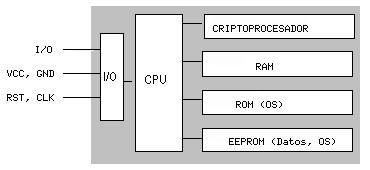
\includegraphics{smartcard.png}
\end{center}
\caption{Estructura gen\'erica de una {\it smartcard}.}
\label{sc}
\end{figure}
\\En la figura \ref{sc} se muestra la estructura m\'as generalista de una 
tarjeta inteligente; en ella podemos observar que el acceso a las \'areas de
memoria s\'olamente es posible a trav\'es de la unidad de entrada/salida y de
una CPU (t\'{\i}picamente de 8 bits), lo que evidentemente aumenta la seguridad 
del dispositivo. Existe tambi\'en
un sistema operativo empotrado en la tarjeta -- generalmente en ROM, aunque 
tambi\'en se puede extender con funciones en la EEPROM -- cuya funci\'on es
realizar tareas criptogr\'aficas (algoritmos de cifrado como RSA o Triple
DES, funciones resumen\ldots); el criptoprocesador apoya estas tareas ofreciendo
operaciones RSA con claves de 512 a 1024 bits. Un ejemplo de implementaci\'on 
real de este esquema lo constituye la tarjeta inteligente CERES, de la F\'abrica
Nacional de Moneda y Timbre espa\~nola (\cite{kn:pit99}); en ella se incluye
adem\'as un generador de n\'umeros aleatorios junto a los mecanismos de 
protecci\'on internos de la tarjeta.\\
\\Cuando el usuario poseedor de una {\it smartcard} desea autenticarse necesita
introducir la tarjeta en un {\it hardware} lector; los dos dispositivos se 
identifican entre s\'{\i} con un protocolo a dos bandas en el que es necesario
que ambos conozcan la misma clave (CK o CCK, {\it Company Key} o {\it Chipcard
Communication Key}), lo que elimina la posibilidad de utilizar tarjetas de
terceros para autenticarse ante el lector de una determinada compa\~n\'{\i}a;
adem\'as esta clave puede utilizarse para asegurar la comunicaci\'on entre
la tarjeta y el dispositivo lector. Tras identificarse las dos partes, se lee
la identificaci\'on personal (PID) de la tarjeta, y el usuario teclea su
PIN; se inicia entonces un protocolo desaf\'{\i}o--respuesta: se env\'{\i}a 
el PID a la m\'aquina y \'esta desaf\'{\i}a a la tarjeta, que responde al
desaf\'{\i}o utilizando una clave personal del usuario (PK, {\it Personal 
Key}). Si la respuesta es correcta, el {\it host} ha identificado la tarjeta y 
el usuario obtiene acceso al recurso pretendido.\\
\\Las ventajas de utilizar tarjetas inteligentes como medio para autenticar
usuarios son muchas frente a las desventajas; se trata de un modelo ampliamente
aceptado entre los usuarios, r\'apido, y que incorpora {\it hardware} de alta
seguridad tanto para almacenar datos como para realizar funciones de cifrado.
Adem\'as, su uso es factible tanto para controles de acceso f\'{\i}sico como 
para controles de acceso l\'ogico a los {\it hosts}, y se integra f\'acilmente 
con otros mecanismos de autenticaci\'on como las contrase\~nas; y en caso de
desear bloquear el acceso de un usuario, no tenemos m\'as que retener su 
tarjeta cuando la introduzca en el lector o marcarla como inv\'alida en una
base de datos (por ejemplo, si se equivoca varias veces al teclar su PIN, igual 
que sucede con una tarjeta de cr\'edito normal). Como principal
inconveniente de las {\it smartcards} podemos citar el coste adicional que
supone para una organizaci\'on el comprar y configurar la infraestructura de
dispositivos lectores y las propias tarjetas; aparte, que un usuario pierda
su tarjeta es bastante f\'acil, y durante el tiempo que no disponga de ella
o no puede acceder al sistema, o hemos de establecer reglas especiales que
pueden comprometer nuestra seguridad (y por supuesto se ha de marcar como 
tarjeta inv\'alida en una base de datos central, para que un potencial atacante
no pueda utilizarla). Tambi\'en la distancia l\'ogica entre la {\it smartcard} y
su poseedor -- simplemente nos podemos fijar en que la tarjeta no tiene
un interfaz para el usuario -- puede ser fuente de varios problemas de
seguridad (\cite{kn:bal99}, \cite{kn:gob96}).\\
\\Aparte de los problemas que puede implicar el uso de {\it smartcards} en 
s\'{\i}, contra la l\'ogica de una tarjeta inteligente existen diversos 
m\'etodos de ataque, como realizar 
ingenier\'{\i}a inversa -- destructiva -- contra el circuito de silicio (y los 
contenidos de la ROM), adulterar la informaci\'on guardada en la tarjeta o 
determinar por diferentes m\'etodos el contenido de la memoria EEPROM. Sin duda
una de las personas que m\'as ha contribuido a incrementar la seguridad de las
{\it smartcards} gracias a sus estudios y ataques es el experto brit\'anico 
Ross J. Anderson (\cite{kn:and97}, \cite{kn:and96}\ldots); en su p\'agina {\it 
web} personal, {\tt http://www.cl.cam.ac.uk/users/rja14/}, podemos encontrar 
todos sus art\'{\i}culos sobre este tema\footnote{Y sobre otros, principalmente 
esteganograf\'{\i}a y criptograf\'{\i}a.}, demasiados como para citarlos 
aqu\'{\i} uno a uno.
\section{Sistemas de autenticaci\'on biom\'etrica}
A pesar de la importancia de la criptolog\'{\i}a en cualquiera de los sistemas 
de 
identificaci\'on de usuarios vistos, existen otra clase de sistemas en los que 
no se aplica esta ciencia, o al menos su aplicaci\'on es secundaria. Es m\'as,
parece que en un futuro no muy lejano estos ser\'an los sistemas que se van a 
imponer en la mayor\'{\i}a de situaciones en las que se haga necesario 
autenticar un usuario: son m\'as amigables para el usuario (no va a necesitar 
recordar {\it passwords} o n\'umeros de identificaci\'on complejos, y, como se 
suele decir, el usuario puede olvidar una tarjeta de identificaci\'on en casa, 
pero nunca se olvidar\'a de su mano o su ojo) y son mucho m\'as 
dif\'{\i}ciles de falsificar que una simple contrase\~na o una tarjeta 
magn\'etica; las principales razones por la que no se han impuesto ya
en nuestros dias es su elevado precio, fuera del alcance de muchas 
organizaciones, y su dificultad de mantenimiento (\cite{kn:gue97}).\\
\\Estos sistemas son los denominados {\bf biom\'etricos}, basados en 
caracter\'{\i}sticas f\'{\i}sicas del usuario a identificar. El reconocimiento 
de formas, la inteligencia artificial y el aprendizaje son las ramas de la 
inform\'atica que desempe\~nan el papel m\'as importante en los sistemas de 
identificaci\'on biom\'etricos; la criptolog\'{\i}a se limita aqu\'{\i} a un uso
secundario, como el cifrado de una base de datos de patrones retinales, o la 
transmisi\'on de una huella dactilar entre un dispositivo analizador y una base
de datos.
La autenticaci\'on basada en caracter\'{\i}sticas f\'{\i}sicas existe desde 
que existe el hombre y, sin darnos cuenta, es la que m\'as utiliza cualquiera
de nosotros en su vida cotidiana: a diario identificamos a personas por los
rasgos de su cara o por su voz. Obviamente aqu\'{\i} el agente reconocedor lo
tiene f\'acil porque es una persona, pero en el modelo aplicable a redes o 
sistemas Unix el agente ha de ser un 
dispositivo que, bas\'andose en caracter\'{\i}sticas del sujeto a identificar,
le permita o deniegue acceso a un determinado recurso.\\
\begin{table}
\begin{center}
\begin{tabular}{|p{0.75in}||p{0.75in}|p{0.75in}|p{0.70in}|p{0.85in}|p{0.65in}|p{0.85in}|}
\hline
& Ojo -- Iris & Ojo -- Retina & Huellas dactilares & Geometr\'{\i}a de la mano & Escritura -- Firma & Voz\\
\hline\hline
Fiabilidad & Muy alta & Muy alta & Alta & Alta & Alta & Alta\\ 
\hline
Facilidad de uso & Media & Baja & Alta & Alta & Alta & Alta\\
\hline
Prevenci\'on de ataques & Muy Alta & Muy alta & Alta & Alta & Media & Media\\
\hline
Aceptaci\'on & Media & Media & Media & Alta & Muy alta & Alta\\
\hline
Estabilidad & Alta & Alta & Alta & Media & Media & Media\\
\hline
Identificaci\'on y autenticaci\'on & Ambas & Ambas & Ambas & Autenticaci\'on & Ambas & Autenticaci\'on\\
\hline
Est\'andars & -- & -- & ANSI/NIST, FBI & -- & -- & SVAPI\\
\hline
Interferencias & Gafas & Irritaciones & Suciedad, heridas, asperezas \ldots & Artritis, reumatismo \ldots & Firmas f\'aciles o cambiantes & Ruido, resfriados \ldots\\
\hline
Utilizaci\'on & Instalaciones nucleares, servicios m\'edicos, centros penitenciarios & Instalaciones nucleares, servicios m\'edicos, centros penitenciarios & Polic\'{\i}a, industrial & General & Industrial & Accesos remotos en bancos o bases de datos\\
\hline 
Precio por nodo en 1997 (USD) & 5000 & 5000 & 1200 & 2100 & 1000 & 1200\\
\hline
\end{tabular}
\end{center}
\caption{Comparaci\'on de m\'etodos biom\'etricos.}
\label{biocomp}
\end{table}
\\Aunque la autenticaci\'on de usuarios mediante m\'etodos biom\'etricos es
posible utilizando cualquier caracter\'{\i}stica \'unica y mesurable del 
individuo (esto incluye desde la forma de teclear ante un ordenador hasta 
los patrones de ciertas venas, pasando por el olor corporal), tradicionalmente 
ha estado basada en cinco grandes grupos (\cite{kn:eve92}). En la tabla 
\ref{biocomp} (\cite{kn:huo98}, \cite{kn:phi97}) se muestra una comparativa de 
sus rasgos m\'as
generales, que vamos a ver con m\'as detalle en los puntos siguientes.\\
\\Los dispositivos biom\'etricos tienen tres partes principales; por un lado,
disponen de un mecanismo autom\'atico que lee y captura una imagen digital o
anal\'ogica de la caracter\'{\i}stica a analizar. Adem\'as disponen de una 
entidad para manejar aspectos como la compresi\'on, almacenamiento o 
comparaci\'on de los datos capturados con los guardados en una base de datos
(que son considerados v\'alidos), y tambi\'en ofrecen una interfaz para las
aplicaciones que los utilizan. El proceso general de autenticaci\'on sigue unos
pasos comunes a todos los modelos de autenticaci\'on biom\'etrica: {\bf 
captura} o lectura de los datos que el usuario a validar presenta, {\bf 
extracci\'on} de ciertas caracter\'{\i}sticas de la muestra (por ejemplo, las
minucias de una huella dactilar), {\bf comparaci\'on} de tales 
caracter\'{\i}sticas con las guardadas en una base de datos, y {\bf decisi\'on}
de si el usuario es v\'alido o no. Es en esta decisi\'on donde principalmente
entran en juego las dos caracter\'{\i}sticas b\'asicas de la fiabilidad de todo
sistema biom\'etrico (en general, de todo sistema de autenticaci\'on): las 
tasas de falso rechazo y de falsa aceptaci\'on. Por tasa de {\bf falso rechazo} 
({\it False Rejection Rate}, FRR) se entiende la probabilidad de que el sistema
de autenticaci\'on rechaze a un usuario leg\'{\i}timo porque no es capaz de
identificarlo correctamente, y por tasa de {\bf falsa aceptaci\'on} ({\it False
Acceptance Rate}, FAR) la probabilidad de que el sistema autentique 
correctamente a un usuario ileg\'{\i}timo; evidentemente, una FRR alta provoca
descontento entre los usuarios del sistema, pero una FAR elevada genera un 
grave problema de seguridad: estamos proporcionando acceso a un recurso a 
personal no autorizado a acceder a \'el.\\
\\Por \'ultimo, y antes de entrar m\'as a fondo con los esquemas de 
autenticaci\'on biom\'etrica cl\'asicos, quiz\'as es conveniente desmentir uno
de los grandes mitos de estos modelos: la vulnerabilidad a ataques de 
simulaci\'on. En cualquier pel\'{\i}cula o libro de esp\'{\i}as que se precie, 
siempre se consigue `enga\~nar' a autenticadores biom\'etricos para conseguir 
acceso a determinadas instalaciones mediante estos ataques: se simula la parte 
del cuerpo a analizar mediante un modelo o incluso utilizando \'organos 
amputados a un cad\'aver o al propio usuario vivo (crudamente, se le corta una 
mano o un dedo, se le saca un ojo\ldots para conseguir que el sistema permita 
la entrada). Evidentemente, esto s\'olo sucede en la ficci\'on: hoy en d\'{\i}a 
cualquier sistema
biom\'etrico -- con excepci\'on, quiz\'as, de algunos modelos basados en voz
de los que hablaremos luego -- son altamente inmunes a estos ataques. Los 
analizadores de retina, de iris, de huellas o de la geometr\'{\i}a de la mano
son capaces, aparte de decidir si el miembro pertenece al usuario leg\'{\i}timo,
de determinar si \'este est\'a vivo o se trata de un cad\'aver.
\subsection{Verificaci\'on de voz}
En los sistemas de reconocimiento de voz no se intenta, como mucha gente piensa,
reconocer lo que el usuario dice, sino identificar una serie de sonidos y sus
caracter\'{\i}sticas para decidir si el usuario es quien dice ser. Para 
autenticar a un usuario utilizando un reconocedor de voz se debe disponer de 
ciertas condiciones para el correcto registro de los datos, como ausencia de 
ruidos, reverberaciones o ecos; idealmente, estas condiciones han de ser las 
mismas siempre que se necesite la autenticaci\'on.\\
\\Cuando un usuario desea acceder al sistema pronunciar\'a unas frases en las
cuales reside gran parte de la seguridad del protocolo; en algunos modelos, los
denominados de texto dependiente, el sistema tiene almacenadas un conjunto muy
limitado de frases que es capaz de reconocer: por ejemplo, imaginemos que el
usuario se limita a pronunciar su nombre, de forma que el reconocedor lo 
entienda y lo autentique. Como veremos a continuaci\'on, estos modelos 
proporcionan poca seguridad en comparaci\'on con los de texto independiente, 
donde el sistema va `proponiendo' a la persona la pronunciaci\'on de ciertas 
palabras
extra\'{\i}das de un conjunto bastante grande. De cualquier forma, sea cual sea
el modelo, lo habitual es que las frases o palabras sean caracter\'{\i}sticas
para maximizar la cantidad de datos que se pueden analizar (por ejemplo, 
frases con una cierta entonaci\'on, pronunciaci\'on de los diptongos, palabras 
con muchas vocales\ldots). Conforme va hablando el usuario, el sistema registra
toda la informaci\'on que le es \'util; cuando termina la frase, ya ha de estar
en disposici\'on de facilitar o denegar el acceso, en funci\'on de la 
informaci\'on analizada y contrastada con la de la base de datos.\\
\\El principal problema del reconocimiento de voz es la inmunidad frente a {\it 
replay attacks}, un modelo de ataques de simulaci\'on en los que un atacante
reproduce (por ejemplo, por medio de un magnet\'ofono) las frases o palabras que
el usuario leg\'{\i}timo pronuncia para acceder al sistema. Este problema es 
especialmente grave en los sistemas que se basan en textos
preestablecidos: volviendo al ejemplo anterior, el del nombre de cada usuario, 
un atacante no tendr\'{\i}a m\'as que grabar a una persona que pronuncia su
nombre ante el autenticador y luego reproducir ese sonido para conseguir el 
acceso; casi la \'unica soluci\'on consiste en utilizar otro sistema de 
autenticaci\'on junto al reconocimiento de voz. Por contra, en modelos de
texto independiente, m\'as interactivos, este ataque no es tan
sencillo porque la autenticaci\'on se produce realmente por una especie de 
desaf\'{\i}o--respuesta entre el usuario y la m\'aquina, de forma que la 
cantidad de texto grabado habr\'{\i}a de ser mucho mayor -- y la velocidad para
localizar la parte del texto que el sistema propone habr\'{\i}a de ser
elevada --. Otro grave problema de los sistemas basados en reconocimiento de
voz es el tiempo que el usuario 
emplea hablando delante del analizador, al que se a\~nade el que \'este necesita
para extraer la informaci\'on y contrastarla con la de su base de datos; aunque
actualmente en la mayor\'{\i}a de sistemas basta con una sola frase, es 
habitual que el usuario se vea obligado a repetirla porque el sistema le deniega
el acceso (una simple congesti\'on hace variar el tono de voz, aunque sea 
levemente, y el sistema no es capaz de decidir si el acceso ha de ser autorizado
o no; incluso el estado an\'{\i}mico de una persona var\'{\i}a su timbre\ldots).
A su favor, el reconocimiento de voz posee la cualidad de una excelente acogida
entre los usuarios, siempre y cuando su funcionamiento sea correcto y \'estos
no se vean obligados a repetir lo mismo varias veces, o se les niegue un acceso
porque no se les reconoce correctamente.
\subsection{Verificaci\'on de escritura}  
Aunque la escritura (generalmente la firma) no es una caracter\'{\i}stica 
estrictamente biom\'etrica, como hemos comentado en la introducci\'on se suele 
agrupar dentro de esta categor\'{\i}a; de la misma forma que suced\'{\i}a en
la verificaci\'on de la voz, el objetivo aqu\'{\i} no es interpretar o entender 
lo que el usuario escribe en el lector, sino autenticarlo bas\'andose en 
ciertos rasgos tanto de la firma como de su r\'ubrica.\\
\\La verificaci\'on en base a firmas es algo que todos utilizamos y aceptamos 
d\'{\i}a a d\'{\i}a en documentos o cheques; no obstante, 
existe una diferencia fundamental entre el uso de las firmas que hacemos en
nuestra vida cotidiana y los sistemas biom\'etricos; mientras que habitualmente 
la verificaci\'on de la firma consiste en un simple an\'alisis visual sobre una 
impresi\'on en papel, est\'atica, en los sistemas autom\'aticos no es posible
autenticar usuarios en base a la representaci\'on de los trazos de su firma. En
los modelos biom\'etricos se utiliza adem\'as la forma de firmar, las 
caracter\'{\i}sticas din\'amicas (por eso se les suele denominar {\it Dynamic
Signature Verification}, DSV): el tiempo utilizado para rubricar, las veces que
se separa el bol\'{\i}grafo del papel, el \'angulo con que se realiza cada
trazo\ldots\\
\\Para utilizar un sistema de autenticaci\'on basado en firmas se solicita en 
primer lugar a los futuros usuarios un n\'umero determinado de firmas ejemplo, 
de las cuales el sistema extrae y almacena ciertas caracter\'{\i}sticas; esta 
etapa se denomina de {\it aprendizaje}, y el principal obst\'aculo a su correcta
ejecuci\'on son los usuarios que no suelen firmar uniformemente. Contra este
problema la \'unica soluci\'on (aparte de una concienciaci\'on de tales 
usuarios) es relajar las restricciones del sistema a la hora de {\it aprender}
firmas, con lo que se decrementa su seguridad.\\
\\Una vez que el sistema conoce las firmas de sus usuarios, cuando estos desean
acceder a \'el se les solicita tal firma, con un n\'umero limitado de intentos
(generalmente m\'as que los sistemas que autentican mediante contrase\~nas, ya
que la firma puede variar en un individuo por m\'ultiples factores). La firma
introducida es capturada por un l\'apiz \'optico o por una lectora sensible
(o por ambos), y el acceso al sistema se produce una vez que el usuario ha 
introducido una firma que el verificador es capaz de distinguir como 
aut\'entica.
\subsection{Verificaci\'on de huellas}  
T\'{\i}picamente la huella dactilar de un individuo ha sido un patr\'on bastante
bueno para determinar su identidad de forma inequ\'{\i}voca, ya que est\'a
aceptado que dos dedos nunca poseen huellas similares, ni siquiera entre 
gemelos o
entre dedos de la misma persona. Por tanto, parece obvio que las huellas
se convertir\'{\i}an antes o despu\'es en un modelo de autenticaci\'on 
biom\'etrico: desde el siglo pasado hasta nuestros d\'{\i}as se vienen 
realizando con \'exito clasificaciones sistem\'aticas de huellas dactilares en 
entornos policiales, y el uso de estos patrones fu\'e uno de los primeros en
establecerse como modelo de autenticaci\'on biom\'etrica.\\
\begin{figure}[t]
\begin{center}
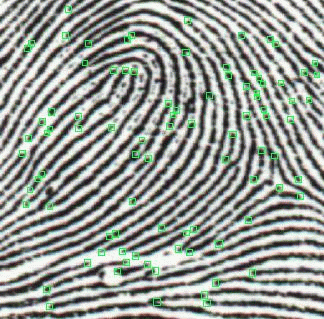
\includegraphics{fingerprint.png}
\end{center}
\caption{Huella dactilar con sus minucias extra\'{\i}das. \copyright 1998 Idex 
AS, {\tt http://www.idex.no/}.}
\label{fingerprint}
\end{figure}
\\Cuando un usuario desea autenticarse ante el sistema situa su dedo en un 
\'area determinada (\'area de lectura, no se necesita en ning\'un momento una 
impresi\'on en tinta). Aqu\'{\i} se toma una imagen que posteriormente se 
normaliza mediante un sistema de finos espejos\footnote{Existen otros m\'etodos
para obtener una imagen de la huella, como la representaci\'on t\'ermica, pero 
su uso es menos habitual -- principalmente por el precio de los lectores --.} 
para corregir \'angulos, y es de
esta imagen normalizada de la que el sistema extrae las minucias (ciertos arcos,
bucles o remolinos de la huella) que va a comparar contra las que tiene en su
base de datos; es importante resaltar que lo que el sistema es capaz de analizar
no es la huella en s\'{\i} sino que son estas minucias, concretamente la 
posici\'on relativa de cada una de ellas. Est\'a demostrado que dos dedos nunca
pueden poseer m\'as de ocho minucias comunes, y cada uno tiene al menos 30 o
40 de \'estas (en la figura \ref{fingerprint} podemos ver una imagen
de una huella digitalizada con sus minucias). Si la comparaci\'on de las 
posiciones relativas de las minucias le\'{\i}das con las almacenadas en la base 
de datos es correcta, se permite el acceso al usuario, deneg\'andosele 
obviamente en caso contrario.\\
\\Los sistemas basados en reconocimiento de huellas son relativamente baratos 
(en comparaci\'on con otros bio\-m\'e\-tri\-cos, como los basados en patrones 
retinales); sin embargo, tienen en su contra la incapacidad temporal de 
autenticar usuarios que se hayan podido herir en el dedo a reconocer (un 
peque\~no corte o una quemadura que afecte a varias minucias pueden hacer
in\'util al sistema). Tambi\'en elementos como la suciedad del dedo, la 
presi\'on ejercida sobre el lector o el estado de la piel pueden ocasionar 
lecturas err\'oneas. Otro factor a tener muy en cuenta contra estos sistemas es
psicol\'ogico, no t\'ecnico: hemos dicho en la introducci\'on que un sistema
de autenticaci\'on de usuarios ha de ser aceptable por los mismos, y 
generalmente el reconocimiento de huellas se asocia a los criminales, por lo que
muchos usuarios recelan del reconocedor y de su uso (\cite{kn:kra97}).
\subsection{Verificaci\'on de patrones oculares}  
Los modelos de autenticaci\'on biom\'etrica basados en patrones oculares se
dividen en dos tecnolog\'{\i}as diferentes: o bien analizan patrones retinales,
o bien analizan el iris. Estos m\'etodos se suelen considerar los m\'as 
efectivos: para una poblaci\'on de 200 millones de potenciales usuarios la 
probabilidad de coincidencia es casi 0, y adem\'as una vez muerto el individuo 
los tejidos oculares degeneran r\'apidamente, lo que dificulta la falsa 
aceptaci\'on de atacantes que puedan robar este \'organo de un cad\'aver.\\
\\La principal desventaja de los m\'etodos basados en el an\'alisis de patrones
oculares es su escasa aceptaci\'on; el hecho de mirar a trav\'es de 
un binocular (o monocular), necesario en ambos modelos, no es c\'omodo para los 
usuarios, ni aceptable para muchos de ellos: por un lado, los usuarios {\it no 
se f\'{\i}an} de un haz de rayos analizando su ojo\footnote{Aunque en el
caso de los irises existen 
dispositivos capaces de leer a una distancia de varios metros, haciendo el 
proceso menos agresivo.}, y por otro un examen de este
\'organo puede revelar enfermedades o caracter\'{\i}sticas m\'edicas que a 
muchas personas les puede interesar mantener en secreto, como el consumo de 
alcohol o
de ciertas drogas. Aunque los fabricantes de dispositivos lectores aseguran que 
s\'olo se analiza el ojo para obtener patrones relacionados con la 
autenticaci\'on, y en ning\'un caso se viola la privacidad de los usuarios, 
mucha gente no cree esta postura oficial (aparte del hecho de que la 
informaci\'on es procesada v\'{\i}a {\it software}, lo que facilita introducir
modificaciones sobre lo que nos han vendido para que un lector realice otras
tareas de forma enmascarada). Por si esto fuera poco, se trata de sistemas 
demasiado caros para la mayor\'{\i}a de organizaciones, y el proceso de
autenticaci\'on no es todo lo r\'apido que debiera en poblaciones de usuarios
elevadas. De esta forma, su uso se ve reducido casi s\'olo a la 
identificaci\'on en sistemas de alta seguridad, como el control de acceso a 
instalaciones militares.
\subsubsection{Retina}
La vasculatura retinal (forma de los vasos sangu\'{\i}neos de la retina humana)
es un elemento ca\-rac\-ter\'{\i}stico de cada individuo, por lo que numerosos
estudios en el campo de la autenticaci\'on de usuarios se basan en el
reconocimiento de esta vasculatura.\\
\\En los sistemas de autenticaci\'on basados en patrones retinales el usuario
a identificar ha de mirar a trav\'es de unos binoculares, ajustar la distancia
interocular y el movimiento de la cabeza, mirar a un punto determinado y por
\'ultimo pulsar un bot\'on para indicar al
dispositivo que se encuentra listo para el an\'alisis. En ese momento se escanea
la retina con una radiaci\'on infrarroja de baja intensidad en forma de espiral,
detectando los nodos y ramas del \'area retinal para compararlos con los 
almacenados en una base de datos; si la muestra coincide con la almacenada para
el usuario que el individuo dice ser, se permite el acceso.\\
\\La compa\~n\'{\i}a EyeDentify posee la patente mundial para analizadores de
vasculatura retinal, por lo que es la principal desarrolladora de esta 
tecnolog\'{\i}a; su p\'agina {\it web} se puede encontrar en {\tt 
http://www.eyedentify.com/}.
\subsubsection{Iris}
El iris humano (el anillo que rodea la pupila, que a simple vista diferencia 
el color de ojos de cada persona) es igual que la vasculatura retinal una 
estructura \'unica por individuo que
forma un sistema muy complejo -- de hasta 266 grados de libertad -- , 
inalterable durante toda la vida de la persona. El uso por parte de un atacante
de \'organos replicados o simulados para conseguir una falsa aceptaci\'on es 
casi imposible con an\'alisis infrarrojo, capaz de detectar con una alta 
probabilidad si el iris es natural o no.\\
\begin{figure}[t]
\begin{center}
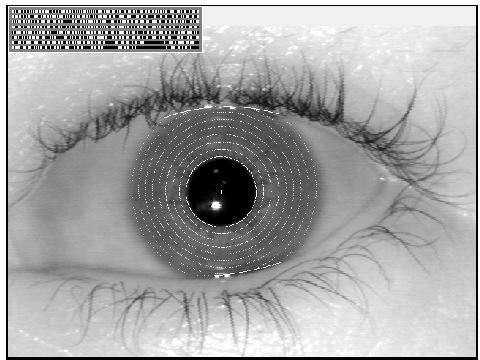
\includegraphics[width=\textwidth]{iriscode.png}
\end{center}
\caption{Iris humano con la extracci\'on de su {\it iriscode}.}
\label{iriscode}
\end{figure}
\\La identificaci\'on basada en el reconocimiento de iris es m\'as moderna que
la basada en patrones retinales; desde hace unos a\~nos el iris humano se viene 
utilizando para la autenticaci\'on de usuarios (\cite{kn:bou96}, 
\cite{kn:dau97}). Para ello, se captura una imagen del iris en blanco
y negro, en un entorno correctamente iluminado; esta imagen se somete a 
deformaciones pupilares (el tama\~no de la pupila var\'{\i}a enormemente en
funci\'on de factores externos, como la luz) y de ella se extraen patrones, que
a su vez son sometidos a transformaciones matem\'aticas (\cite{kn:mcm97}) hasta 
obtener una 
cantidad de datos (t\'{\i}picamente 256 {\it KBytes}) suficiente para
los prop\'ositos de autenticaci\'on. Esa muestra, denominada {\it iriscode} 
(en la figura \ref{iriscode} se muestra una imagen de un iris humano con su 
{\it iriscode} asociado) es comparada con otra tomada
con anterioridad y almacenada en la base de datos del sistema, de forma que si
ambas coinciden el usuario se considera autenticado con \'exito; la 
probabilidad de una falsa aceptaci\'on es la menor de todos los modelos
biom\'etricos (\cite{kn:dau98}).\\
\\La empresa estadounidense {\it IriScan} es la principal desarrolladora de
tecnolog\'{\i}a (y de investigaciones) basada en reconocimiento de iris que
existe actualmente, ya que posee la patente sobre esta tecnolog\'{\i}a; 
su p\'agina {\it web}, con interesantes art\'{\i}culos sobre este modelo de 
autenticaci\'on (a diferencia de la p\'agina de EyeDentify), se puede consultar 
en {\tt http://www.iriscan.com/}.
\subsection{Verificaci\'on de la geometr\'{\i}a de la mano}
\begin{figure}[t]
\begin{center}
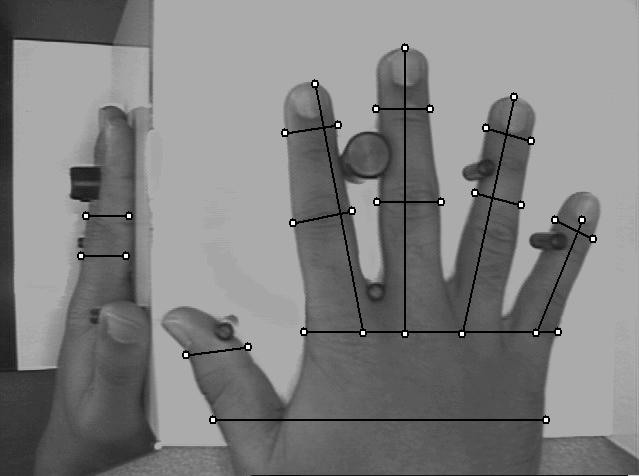
\includegraphics[width=\textwidth]{hand.png}
\end{center}
\caption{Geometr\'{\i}a de una mano con ciertos par\'ametros extra\'{\i}dos.}
\label{hand}
\end{figure}
Los sistemas de autenticaci\'on basados en el an\'alisis de la geometr\'{\i}a
de la mano son sin duda los m\'as r\'apidos dentro de los biom\'etricos: con
una probabilidad de error aceptable en la mayor\'{\i}a de ocasiones, en 
aproximadamente un 
segundo son capaces de determinar si una persona es quien dice ser.\\
\\Cuando un usuario necesita ser autenticado situa su mano sobre un dispositivo
lector con unas gu\'{\i}as que marcan la posici\'on correcta para la lectura
(figura \ref{hand}). Una vez la mano est\'a correctamente situada, unas 
c\'amaras toman una imagen superior y otra lateral, de las que se extraen 
ciertos datos (anchura, longitud, \'area, determinadas distancias\ldots) en un 
formato de tres dimensiones. Transformando estos datos en un modelo 
matem\'atico que se contrasta contra una base de patrones, el sistema es capaz
de permitir o denegar acceso a cada usuario.\\
\\Quiz\'as uno de los elementos m\'as importantes del reconocimiento mediante
analizadores de geometr\'{\i}a de la mano es que \'estos son capaces de 
aprender: a la vez que autentican a un usuario, actualizan su base de datos con
los cambios que se puedan producir en la muestra (un peque\~no crecimiento, 
adelgazamiento, el proceso de cicatrizado de una herida\ldots); de esta forma
son capaces de identificar correctamente a un usuario cuya muestra se tom\'o 
hace a\~nos, pero que ha ido accediendo al sistema con regularidad. Este hecho, 
junto a su rapidez y su buena aceptaci\'on entre los usuarios, hace que los 
autenticadores basados en la geometr\'{\i}a de la mano sean los m\'as 
extendidos dentro de los biom\'etricos a pesar de que su tasa de falsa
aceptaci\'on se podr\'{\i}a considerar inaceptable en algunas situaciones: no
es normal, pero s\'{\i} posible, que dos personas tengan la mano lo 
suficientemente parecida como para que el sistema las confunda. Para minimizar
este problema se recurre a la identificaci\'on basada en la geometr\'{\i}a de
uno o dos dedos, que adem\'as puede usar dispositivos lectores m\'as baratos y
proporciona incluso m\'as rapidez.
\section{Autenticaci\'on de usuarios en Unix}
\label{unixua}
\subsection{Autenticaci\'on cl\'asica}
En un sistema Unix habitual cada usuario posee un nombre de entrada al sistema
o {\it login} y una clave o {\it password}; ambos datos se almacenan 
generalmente en el fichero {\tt /etc/passwd}. Este archivo contiene una 
l\'{\i}nea por usuario (aunque hay entradas que no corresponden a usuarios 
reales, como veremos a continuaci\'on) donde se indica la informaci\'on 
necesaria para que los usuarios puedan conectar al sistema y trabajar en \'el, 
separando los diferentes campos mediante {\tt `:'}. Por ejemplo, podemos
encontrar entradas parecidas a la siguiente:
\begin{center}
{\tt toni:LEgPN8jqSCHCg:1000:100:Antonio Villalon,,,:/export/home/toni:/bin/sh}\vspace{5pt}\\
\end{center}
En primer lugar aparecen el {\it login} del usuario y su clave cifrada; a 
continuaci\'on tenemos dos n\'umeros que ser\'an el identificador de usuario y
el de grupo respectivamente. El quinto campo, denominado {\sc gecos} es 
simplemente informaci\'on administrativa sobre la identidad real del usuario,
como su nombre, tel\'efono o n\'umero de despacho. Finalmente, los dos \'ultimos
campos corresponden al directorio del usuario (su {\it \$HOME} inicial) y al
{\it shell} que le ha sido asignado.\\
\\Al contrario de lo que mucha gente cree, Unix no es capaz de distinguir a sus
usuarios por su nombre de entrada al sistema. Para el sistema operativo lo que
realmente distingue a una persona de otra (o al menos a un usuario de otro) es
el UID del usuario en cuesti\'on; el {\it login} es algo que se 
utiliza principalmente para comodidad de las personas (obviamente es m\'as 
f\'acil acordarse de un nombre de entrada como {\it toni} que de un UID como 
2643, sobre todo si se tienen cuentas en varias m\'aquinas, cada una con un UID 
diferente). Por tanto, si en {\tt /etc/passwd} existen
dos entradas con un mismo UID, para Unix se tratar\'a del mismo usuario, aunque
tengan un {\it login} y un {\it password} diferente: as\'{\i}, si dos usuarios
tienen asignado el UID 0, ambos tendr\'an privilegios de superusuario, sin
importar el {\it login} que utilicen. Esto es especialmente aprovechado por 
atacantes que han
conseguido privilegios de administrador en una m\'aquina: pueden a\~nadir una 
l\'{\i}nea a {\tt /etc/passwd} mezclada entre todas las dem\'as, con un nombre 
de usuario normal pero con el UID 0; as\'{\i} garantizan su entrada al sistema 
como administradores en caso de ser descubiertos, por ejemplo para borrar 
huellas. Como a simple vista puede resultar dif\'{\i}cil localizar la 
l\'{\i}nea insertada, especialmente en sistemas con un gran n\'umero de 
usuarios, para detectar las cuentas con privilegios en la m\'aquina podemos 
utilizar la siguiente orden:
\begin{quote} 
\begin{verbatim} 
anita:~# awk -F: '$3==0 {print $1}' /etc/passwd
root
anita:~#
\end{verbatim}
\end{quote}\vspace{5pt}
En el fichero de claves van a existir entradas que no corresponden a usuarios
reales, sino que son utilizadas por ciertos programas o se trata de cuentas 
mantenidas por motivos de compatibilidad con otros sistemas; t\'{\i}picos 
ejemplos de este tipo de entradas son {\tt lp}, {\tt uucp} o {\tt postmaster}.
Estas cuentas han de estar bloqueadas en la mayor\'{\i}a de casos, para evitar
que alguien pueda utilizarlas para acceder a nuestro sistema: s\'olo han de
ser accesibles para el {\it root} mediante la orden {\tt su}. Aunque en su 
mayor\'{\i}a cumplen esta condici\'on, en algunos sistemas estas cuentas tienen
claves por defecto o, peor, no tienen claves, lo que las convierte en una 
puerta completamente abierta a los intrusos; es conveniente que, una vez 
instalado el sistema operativo, y antes de poner a trabajar la m\'aquina, 
comprobemos que est\'an bloqueadas, o en su defecto que tienen claves no 
triviales. Algunos ejemplos de cuentas sobre los que hay que prestar una 
especial atenci\'on son\footnote{Hemos preferido no mostrar las claves por 
defecto (si las tienen) ni el sistema operativo concreto.} {\tt root}, 
{\tt guest}, {\tt lp}, {\tt demos}, {\tt 4DGifts}, {\tt tour}, {\tt uucp}, 
{\tt nuucp}, {\tt games} o {\tt postmaster}; es muy recomendable
consultar los manuales de cada sistema concreto, y chequear peri\'odicamente 
la existencia de cuentas sin clave o cuentas que deber\'{\i}an permanecer 
bloqueadas y no lo est\'an.\\  
\\Para cifrar las claves de acceso de sus usuarios, el sistema operativo
Unix emplea un criptosistema irreversible que utiliza la funci\'on est\'andar
de C {\tt crypt(3)}, basada en el algoritmo DES. Para una 
descripci\'on exhaustiva del funcionamiento de {\tt crypt(3)} se puede consultar
\cite{kn:mor79}, \cite{kn:fel90} o \cite{kn:spa96}. Esta funci\'on
toma como clave los ocho primeros caracteres de la contrase\~na elegida por el 
usuario (si la longitud de \'esta es menor, se completa con ceros) para cifrar 
un bloque de 
texto en claro de 64 bits puestos a cero; para evitar que dos {\it passwords}
iguales resulten en un mismo texto cifrado, se realiza una permutaci\'on durante
el proceso de cifrado elegida de forma autom\'atica y aleatoria para cada 
usuario, basada en un campo formado por un n\'umero de 12 bits (con lo que
conseguimos 4096 permutaciones diferentes) llamado {\it salt}.
El cifrado resultante se vuelve a cifrar utilizando la contrase\~na del 
usuario de nuevo como clave, y permutando con el mismo {\it salt}, 
repiti\'endose el 
proceso 25 veces. El bloque cifrado final, de 64 bits, se concatena con dos 
bits cero, obteniendo 66 bits que se hacen representables en 11 caracteres de 6 
bits cada uno y que, junto con el {\it salt}, pasan a constituir el campo {\it 
password} del fichero de contrase\~nas, usualmente {\tt /etc/passwd}. As\'{\i}, 
los dos primeros caracteres de este campo estar\'an constituidos por el {\it 
salt} y los 11 restantes por la contrase\~na cifrada:
\begin{center}
{\tt toni:{\bf LEgPN8jqSCHCg}:1000:100:Antonio Villalon,,,:/export/home/toni:/bin/sh}\vspace{5pt}\\
{\sc salt:} \fbox{LE}\hspace{50pt}
{\sc Password cifrado:} \fbox{gPN8jqSCHCg}
\end{center}
Como hemos dicho antes, este criptosistema es irreversible. Entonces, >c\'omo 
puede un usuario conectarse a una m\'aquina Unix? El proceso es sencillo: el 
usuario 
introduce su contrase\~na, que se utiliza como clave para cifrar 64 bits a 0
bas\'andose en el {\it salt}, le\'{\i}do en {\tt /etc/passwd}, de dicho usuario.
Si tras aplicar el algoritmo de 
cifrado el resultado se corresponde con lo almacenado en los \'ultimos 11 
caracteres del campo {\it password} del fichero de contrase\~nas, la clave del 
usuario se considera v\'alida y se permite el acceso. En caso contrario se le
deniega y se almacena en un fichero el intento de conexi\'on fallido.
\subsection{Mejora de la seguridad}
\subsubsection{Problemas del modelo cl\'asico}
Los ataques de texto cifrado escogido constituyen la principal amenaza al 
sistema de 
autenticaci\'on de Unix; a diferencia de lo que mucha gente cree, no es posible 
descifrar una contrase\~na, pero es muy f\'acil cifrar una palabra junto a un
determinado {\it salt}, y comparar el resultado con la cadena almacenada en el 
fichero de claves. De esta forma, un atacante leer\'a el fichero {\tt 
/etc/passwd} (este fichero ha de tener permiso de lectura para todos los 
usuarios si queremos que el sistema funcione correctamente), y mediante un 
programa adivinador (o {\it crackeador}) como {\tt Crack} o {\tt John the 
Ripper} cifrar\'a todas 
las palabras de un fichero denominado {\it diccionario} (un fichero ASCII con 
un gran n\'umero de palabras de cualquier idioma o campo de la sociedad -- 
historia cl\'asica, deporte, cantantes de {\it rock}\ldots), comparando el 
resultado obtenido en este proceso con la clave cifrada del fichero de 
contrase\~nas; si ambos coinciden, ya ha obtenido una clave para acceder al 
sistema de forma no autorizada. Este proceso se puede pero no se suele hacer en 
la m\'aquina local, ya que en este caso hay bastantes posibilidades de detectar 
el ataque: desde modificar en c\'odigo de la funci\'on {\tt crypt(3)} para que
alerte al administrador cuando es invocada repetidamente (cada vez que el 
adivinador cifra una palabra utiliza esta funci\'on) hasta simplemente darse 
cuenta de una carga de CPU excesiva (los programas adivinadores suelen consumir 
un tiempo de procesador considerable). Lo habitual es que el atacante transfiera
una copia del archivo a otro ordenador y realice el proceso en esta otra 
m\'aquina; ni siquiera se tiene que tratar de un servidor Unix con gran 
capacidad de c\'omputo: existen muchos programas adivinadores que se ejecutan 
en un PC normal, bajo MS-DOS o Windows. Obviamente, este segundo caso es mucho
m\'as dif\'{\i}cil de detectar, ya que se necesita una auditor\'{\i}a de los
programas que ejecuta cada usuario (y utilidades como {\tt cp} o {\tt ftp} no
suelen llamar la atenci\'on del administrador). Esta auditor\'{\i}a la ofrecen
muchos sistemas Unix (generalmente en los ficheros de {\it log} {\tt 
/var/adm/pacct} o {\tt /var/adm/acct}), pero no se suele utilizar por los 
excesivos recursos que puede consumir, incluso en sistemas peque\~nos; 
obviamente, no debemos fiarnos nunca de los archivos hist\'oricos de \'ordenes 
del usuario (como {\tt \$HOME/.sh$\_$history} o {\tt \$HOME/.bash$\_$history}), 
ya que el atacante los puede modificar para ocultar sus actividades, sin 
necesidad de ning\'un privilegio especial.
\subsubsection{Contrase\~nas aceptables}
La principal forma de evitar este tipo de ataque es utilizar {\it passwords} 
que no sean palabras de los ficheros {\it diccionario} t\'{\i}picos: 
combinaciones de min\'usculas y may\'usculas, n\'umeros mezclados con texto, 
s\'{\i}mbolos como \&, \$ o \%, etc. Por supuesto, hemos de huir de claves
simples como {\it internet} o {\it beatles}, nombres propios, combinaciones 
d\'ebiles como {\it Pepito1} o {\it qwerty}, nombres de lugares, actores, 
personajes de libros, deportistas\ldots Se han realizado numerosos estudios
sobre c\'omo evitar este tipo de {\it passwords} en los usuarios 
(\cite{kn:alv88}, \cite{kn:kle90}, \cite{kn:spa91b}, \cite{kn:bel93}, 
\cite{kn:bis91}, \cite{kn:bis95}\dots), y tambi\'en se han dise\~nado potentes 
herramientas para lograrlo, como {\tt Npasswd} o {\tt Passwd+} 
(\cite{kn:spa91b}, \cite{kn:bis92}, \cite{kn:che92}\ldots). Es bastante 
recomendable instalar alguna de ellas para `obligar' a los usuarios a utilizar
contrase\~nas aceptables (muchos Unices ya las traen incorporadas), pero 
no conviene confiar toda la seguridad de nuestro sistema a estos 
programas\footnote{<Ni a ning\'un otro!}.
Como norma, cualquier administrador deber\'{\i}a ejecutar con cierta 
periodicidad alg\'un programa adivinador, tipo {\it Crack}, para comprobar que
sus usuarios no han elegidos contrase\~nas d\'ebiles (a pesar del uso de 
{\tt Npasswd} o {\tt Passwd+}): se puede tratar de claves generadas antes de
instalar estas utilidades o incluso de claves asignadas por el propio {\it root}
que no han pasado por el control de estos programas.\\%\vspace{6pt}\\
\\Por \'ultimo es necesario recordar que para que una contrase\~na sea aceptable
obligatoriamente ha de cumplir el principio {\bf KISS}, que hablando de {\it
passwords} est\'a claro que no puede significar {\it `Keep it simple, stupid!'}
sino {\bf `Keep it SECRET, stupid!'}. La contrase\~na m\'as larga, la m\'as
dif\'{\i}cil de recordar,
la que combina m\'as caracteres no alfab\'eticos\ldots pierde toda su robustez
si su propietario la comparte con otras personas\footnote{{\it `Three can keep
a secret\ldots if two of them are dead'}. Benjamin Franklin.}.
\begin{center}
\fbox{
\parbox{5.5in}{
Para verificar el hecho que de no hay que confiar toda la seguridad de un 
sistema a ning\'un programa, hemos {\it crackeado} el fichero de claves de un
servidor de la Universidad Polit\'ecnica de Valencia. Se trata de un sistema 
Unix con unos 1300 
usuarios, dedicado a c\'alculo cient\'{\i}fico (obviamente, no vamos a decir
el nombre del servidor). A pesar de utilizar un mecanismo que no permite que
los usuarios elijan claves d\'ebiles, en menos de dos horas de ejecuci\'on sobre
un Pentium MMX a 233 MHz el programa Crack corriendo sobre Solaris ha encontrado
seis claves de usuario utilizando exclusivamente diccionarios de demostraci\'on 
que acompa\~nan al programa (seguramente si utiliz\'aramos diccionarios en 
castellano o relacionados con temas como el deporte o la m\'usica nacionales
-- que los hay-- habr\'{\i}amos encontrado alguna clave m\'as\ldots). Se puede 
pensar que s\'olo seis usuarios de entre 1300 es 
algo bastante aceptable, pero no es as\'{\i}: cualquier combinaci\'on v\'alida
de {\it login} y {\it password} es una puerta abierta en nuestro sistema; si
un intruso consigue entrar por esta puerta, tiene m\'as del 70\% del camino
recorrido para obtener el control total de la m\'aquina. Si queremos conseguir
un sistema m\'{\i}nimamente fiable, no podemos permitir ni una sola clave 
d\'ebil.\\
Sin embargo, tampoco hay que pensar que programas como {\tt Passwd+} no 
desempe\~nan bien su labor: en 1994, cuando en el sistema con el que hemos 
realizado la prueba anterior no dispon\'{\i}a de estos mecanismos de seguridad,
en menos de 12 horas de ejecuci\'on de un programa adivinador sobre un 486DX a
33 MHz utilizando Linux, se consiguieron extraer m\'as de cien claves, entre
ellas algunas de usuarios con cierto nivel de privilegio dentro del sistema.
}}\vspace{10pt}
\end{center}
\subsubsection{Shadow Password}
Otro m\'etodo cada d\'{\i}a m\'as utilizado para proteger las contrase\~nas
de los usuarios el denominado {\it Shadow Password} u oscurecimiento de
contrase\~nas. La idea b\'asica de 
este mecanismo es impedir que los usuarios sin privilegios puedan leer el 
fichero donde se almacenan las claves cifradas; en el punto anterior hemos
comentado que el fichero {\tt /etc/passwd} tiene que tener permiso de lectura
para todo el mundo si queremos que el sistema funcione correctamente. En 
equipos con oscurecimiento de contrase\~nas este fichero sigue siendo legible
para todos los usuarios, pero a diferencia del mecanismo tradicional, las 
claves cifradas no se guardan en \'el, sino en el archivo {\tt /etc/shadow},
que s\'olo el {\it root} puede leer. En el campo correspondiente a la clave
cifrada de {\tt /etc/passwd} no aparece \'esta, sino un s\'{\i}mbolo que indica
a determinados programas (como {\tt /bin/login}) que han de buscar las claves 
en {\tt /etc/shadow}, generalmente una {\tt x}:
\begin{center}
{\tt toni:{\bf x}:1000:100:Antonio Villalon,,,:/export/home/toni:/bin/sh}\vspace{5pt}\\
\end{center}
El aspecto de {\tt /etc/shadow} es en cierta forma similar al de {\tt 
/etc/passwd} que ya hemos comentado: existe una l\'{\i}nea por cada usuario del
sistema, en la que se almacena su {\it login} y su clave cifrada. Sin embargo, 
el resto de campos de este fichero son diferentes; corresponden a informaci\'on 
que permite implementar otro mecanismo para proteger las claves de los usuarios,
el envejecimiento de contrase\~nas o {\it Aging Password}, del que hablaremos a
continuaci\'on:
\begin{center}
{\tt toni:LEgPN8jqSCHCg:10322:0:99999:7:::}
\end{center}
Desde hace un par de a\~nos, la gran mayor\'{\i}a de Unices del mercado 
incorporan este mecanismo; si al instalar el sistema operativo las claves 
aparecen almacenadas en {\tt /etc/passwd} podemos comprobar si existe la orden
{\tt pwconv}, que convierte un sistema cl\'asico a uno oscurecido. Si no es
as\'{\i}, o si utilizamos un Unix antiguo que no posee el mecanismo de {\it
Shadow Password}, es muy conveniente que consigamos el paquete que lo 
implementa (seguramente se tratar\'a de un fichero {\tt shadow.tar.gz} que
podemos encontar en multitud de servidores, adecuado a nuestro clon de Unix) y
lo instalemos en el equipo. Permitir que todos los usuarios lean las 
claves cifradas ha representado durante a\~nos, y sigue representando, uno de 
los mayores problemas de seguridad de Unix; adem\'as, una de las actividades
preferidas de piratas novatos es intercambiar ficheros de claves de los sistemas
a los que acceden y {\it crackearlos}, con lo que es suficiente una persona que
lea nuestro fichero para tener en poco tiempo una colonia de intrusos en 
nuestro sistema. 
\subsubsection{Envejecimiento de contrase\~nas}
En casi todas las implementaciones de {\it Shadow Password} 
actuales\footnote{{\it AT\&T/USL} fu\'e el pionero en utilizar envejecimiento
junto al {\it shadow password}.} se suele incluir la
implementaci\'on para otro mecanismo de protecci\'on de las claves denominado
envejecimiento de contrase\~nas ({\it Aging Password}). La idea b\'asica de
este mecanismo es proteger los {\it passwords} de los usuarios d\'andoles un 
determinado periodo de vida: una contrase\~na s\'olo va a ser v\'alida durante 
un cierto tiempo, pasado el cual expirar\'a y el usuario deber\'a cambiarla.\\
\\Realmente, el envejecimiento previene m\'as que problemas con las claves 
problemas con la transmisi\'on de \'estas por la red: cuando conectamos 
mediante mecanismos como {\tt telnet}, {\tt ftp} o {\tt rlogin} a un sistema 
Unix, cualquier equipo entre el nuestro y el servidor puede leer los paquetes
que enviamos por la red, incluyendo aquellos que contienen nuestro nombre de
usuario y nuestra contrase\~na (hablaremos de esto m\'as a fondo en los 
cap\'{\i}tulos dedicados a la seguridad del sistema de red y a la 
criptograf\'{\i}a); de esta forma, un atacante situado en un ordenador 
intermedio puede obtener muy f\'acilmente nuestro {\it login} y nuestro {\it 
password}. Si la clave capturada es v\'alida indefinidamente, esa persona tiene
un acceso asegurado al servidor en el momento que quiera; sin embargo, si la
clave tiene un periodo de vida, el atacante s\'olo podr\'a utilizarla antes de
que el sistema nos obligue a cambiarla.\\
\\A primera vista, puede parecer que la utilidad del envejecimiento de 
contrase\~nas no es muy grande; al fin y al cabo, la lectura de paquetes 
destinados a otros equipos ({\it sniffing}) no se hace por casualidad: el 
atacante que lea la red en busca de claves y nombres de usuario lo va a hacer
porque quiere utilizar estos datos contra un sistema. Sin embargo, una 
pr\'actica habitual es dejar programas escuchando durante d\'{\i}as y grabando 
la informaci\'on le\'{\i}da en ficheros; cada cierto tiempo el pirata 
consultar\'a los resultados de tales programas, y si la clave le\'{\i}da ya ha 
expirado y su propietario la ha cambiado por otra, el haberla capturado no le 
servir\'a de nada a ese atacante.\\
\begin{figure}[t]
\vspace{0.5in}
\begin{center}
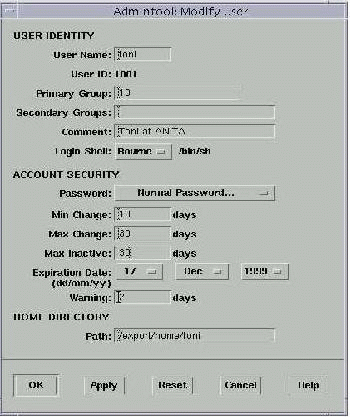
\includegraphics{admintool.png}
\vspace{0.3in}
\end{center}
\caption{La herramienta de administraci\'on {\tt admintool} (Solaris), con
opciones para envejecimiento de claves.}
\label{admintool}
\end{figure}
\\Los periodos de expiraci\'on de las claves se suelen definir a la hora de
crear a los usuarios con las herramientas que cada sistema ofrece para ello
(por ejemplo, Solaris y su {\tt admintool}, mostrado en la figura \ref{admintool}). 
Si queremos modificar alguno de estos periodos una vez establecidos, desde esas
mismas herramientas de administraci\'on podremos hacerlo, y tambi\'en desde
l\'{\i}nea de \'ordenes mediante \'ordenes como {\tt chage} o {\tt usermod}.
Como antes hemos dicho, en el archivo {\tt /etc/shadow} se almacena, junto a la 
clave cifrada de cada usuario, la informaci\'on necesaria para implementar el 
envejecimiento de contrase\~nas; una entrada de este archivo es de la forma
\begin{center}
{\tt toni:LEgPN8jqSCHCg:10322:0:99999:7:::}
\end{center}
Tras el {\it login} y el {\it password} de cada usuario se guardan los campos 
siguientes:
\begin{itemize}
\item D\'{\i}as transcurridos desde el 1 de enero de 1970 hasta que la clave se 
cambi\'o por \'ultima vez.
\item D\'{\i}as que han de transcurrir antes de que el usuario pueda volver a
cambiar su contrase\~na.
\item D\'{\i}as tras los cuales se ha de cambiar la clave.
\item D\'{\i}as durante los que el usuario ser\'a avisado de que su clave va
a expirar antes de que \'esta lo haga.
\item D\'{\i}as que la cuenta estar\'a habilitada tras la expiraci\'on de la
clave.
\item D\'{\i}as desde el 1 de enero de 1970 hasta que la cuenta se deshabilite.
\item Campo reservado.
\end{itemize}
Como podemos ver, cuando un usuario cambia su clave el sistema le impide 
volverla a cambiar durante un periodo de tiempo; con esto se consigue que 
cuando el sistema obligue a cambiar la contrase\~na el usuario no restaure 
inmediatamente su clave antigua (en este caso el esquema no servir\'{\i}a de
nada). Cuando este periodo finaliza, suele existir un intervalo de cambio 
voluntario: est\'a permitido el cambio de contrase\~na, aunque no es 
obligatorio; al finalizar este nuevo periodo, el {\it password} ha expirado y ya
es obligatorio cambiar la clave. Si el n\'umero m\'aximo de d\'{\i}as en los
que el usuario no puede cambiar su contrase\~na es mayor que el n\'umero de 
d\'{\i}as tras los cuales es obligatorio el cambio, el usuario {\bf no puede
cambiar nunca su clave}. Si tras el periodo de cambio obligatorio el {\it
password} permanece inalterado, la cuenta se bloquea.\\
\\En los sistemas Unix m\'as antiguos (hasta {\it System V Release 3.2}), sin 
{\it shadow password}, toda la informaci\'on de envejecimiento se almacena en 
{\tt /etc/passwd}, junto al campo correspondiente a la clave cifrada de cada 
usuario pero separada de \'este por una coma:
\begin{center}
{\tt root:cp5zOHITeZLWM,A.B8:0:0:El Spiritu Santo,,,:/root:/bin/bash}
\end{center}
\begin{table}
\begin{center}
\begin{tabular}{|c||c|c|c|c|c|c|c|c|c|c|c|c|c|c|c|}
\hline
Car\'acter & . & / & 0 & 1 & 2 & 3 & 4 & 5 & 6 & 7 & 8 & 9 & A & B & C\\
\hline
Valor (semanas) & 1 & 2 & 3 & 4 & 5 & 6 & 7 & 8 & 9 & 10 & 11 & 12 & 13 & 14 & 15 \\
\hline
Car\'acter & D & E & F & G & H & I & J & K & L & M & N & O & P & Q & R\\ 
\hline
Valor (semanas) & 16 & 17 & 18 & 19 & 20 & 21 & 21 & 22 & 23 & 24 & 25 & 26 & 27 & 28 & 29\\ 
\hline
Car\'acter & S & T & U & V & W & X & Y & Z & a & b & c & d & e & f & g\\
\hline
Valor (semanas) & 30 & 31 & 32 & 33 & 34 & 35 & 36 & 37 & 38 & 39 & 40 & 41 & 42 & 43 & 44\\ 
\hline
Car\'acter & h & i & j & k & l & m & n & o & p & q & r & s & t & u & v\\
\hline
Valor (semanas) & 45 & 46 & 47 & 48 & 49 & 50 & 51 & 52 & 53 & 54 & 55 & 56 & 57 & 58 & 59\\
\hline
Car\'acter & w & x & y & z &&&&&&&&&&&\\
\hline
Valor (semanas) & 60 & 61 & 62 & 63 &&&&&&&&&&&\\
\hline
\end{tabular}
\end{center}
\caption{C\'odigos de caracteres para el envejecimiento de contrase\~nas.}
\label{agingcodes}
\end{table}
En este caso el primer car\'acter tras la coma es el n\'umero m\'aximo de 
semanas antes de que el {\it password} expire; el siguiente car\'acter es el 
n\'umero m\'{\i}nimo de semanas antes de que el usuario pueda cambiar su clave,
y el tercer y cuarto car\'acter indican el tiempo transcurrido desde el 1 de
enero de 1970 hasta el \'ultimo cambio de contrase\~na. Todos estos tiempos
se indican mediante determinados caracteres con un significado especial, 
mostrados en la tabla \ref{agingcodes}. Tambi\'en se contemplan en este esquema
tres casos especiales: si los dos primeros caracteres son {\tt `..'} el usuario
ser\'a obligado a cambiar su clave la siguiente vez que conecte al sistema; el
programa {\tt passwd} modificar\'a entonces su entrada en el archivo para que
el usuario no se vuelva a ver afectado por el envejecimiento. Otro caso especial
ocurre cuando los dos \'ultimos caracteres tambi\'en son {\tt `..'}, situaci\'on
en la cual el usuario igualmente se ver\'a obligado a cambiar su clave la
pr\'oxima vez que conecte al sistema pero el envejecimiento seguir\'a definido
por los dos primeros caracteres. Por \'ultimo, si el primer car\'acter tras la
coma es menor que el siguiente, el usuario no puede cambiar su {\it password}
nunca, y s\'olo puede ser modificado a trav\'es de la cuenta {\it root}.
\subsubsection{Claves de un solo uso}
El envejecimiento de contrase\~nas tiene dos casos extremos. Por un lado, 
tenemos el esquema cl\'asico: una clave es v\'alida hasta que el usuario 
voluntariamente decida cambiarla (es decir, no hay caducidad de 
la contrase\~na). El extremo contrario del {\it Aging Password} es otorgar un 
tiempo de vida m\'{\i}nimo a cada clave, de forma que s\'olo sirva para una 
conexi\'on: es lo que se denomina clave de un solo uso, {\it One Time Password} 
(\cite{kn:lam81}).\\
\\>C\'omo utilizar contrase\~nas de un s\'olo uso? Para conseguirlo existen
diferentes aproximaciones; la m\'as simplista consiste en asignar al usuario
una lista en papel con la secuencia de claves a utilizar, de forma que cada
vez que \'este conecte al sistema elimina de la lista la contrase\~na que acaba 
de utilizar. Por su parte, el sistema avanza en su registro para que la
pr\'oxima vez que el usuario conecte pueda utilizar la siguiente clave. Otra
aproximaci\'on consiste en utilizar un peque\~no dispositivo que el usuario 
debe llevar consigo, como una tarjeta o una calculadora especial, de forma que
cuando desee conectar el sistema le indicar\'a una secuencia de caracteres a
teclear en tal dispositivo; el resultado obtenido ser\'a lo que se ha de 
utilizar como {\it password}. Para incrementar la seguridad ante un robo de la
tarjeta, antes de teclear el n\'umero recibido desde la m\'aquina suele ser
necesario utilizar un P.I.N. que el usuario debe mantener en secreto 
(\cite{kn:spa96}).\\
\\Una de las implementaciones del {\it One Time Password} m\'as extendida entre
los diferentes clones de Unix es {\sc s/key} (\cite{kn:hal94}), disponible 
tambi\'en para clientes Windows y MacOS. Utilizando este {\it software}, la
clave de los usuarios no viaja nunca por la red, ni siquiera al ejecutar 
\'ordenes como {\tt su} o {\tt passwd}, ni tampoco se almacena informaci\'on
comprometedora (como las claves en claro) en la m\'aquina servidora. Cuando el
cliente desea conectar contra un sistema genera una contrase\~na de un solo
uso, que se verifica en el servidor; en ambas tareas se utilizan las funciones
resumen {\sc md4} (\cite{kn:riv90}) o {\sc md5} (\cite{kn:riv92}). Para realizar
la autenticaci\'on, la m\'aquina servidora guarda una copia del {\it password}
que recibe del cliente y le aplica la funci\'on resumen; si el resultado no
coincide con la copia guardada en el fichero de contrase\~nas, se deniega el
acceso. Si por el contrario la verificaci\'on es correcta se actualiza la 
entrada del usuario en el archivo de claves con el {\it one time password} que
se ha recibido (antes de aplicarle la funci\'on), avanzando as\'{\i} en la
secuencia de contrase\~nas. Este avance decrementa en uno el n\'umero de 
iteraciones de la funci\'on ejecutadas, por lo que ha de llegar un momento 
en el que el usuario debe reiniciar el contador o en caso contrario se le
negar\'a el acceso al sistema; para ello ejecuta una versi\'on modificada de 
la orden {\tt passwd}.
\subsubsection{Otros m\'etodos}
Algo por lo que se ha criticado el esquema de autenticaci\'on de usuarios de
Unix es la longitud -- para prop\'ositos de alta seguridad, demasiado corta --
de sus claves; lo que hace a\~nos era poco m\'as que un planteamiento 
te\'orico (\cite{kn:dif77}), actualmente es algo factible: sin ni siquiera 
entrar en temas de {\it hardware} dedicado, seguramente demasiado caro para la
mayor\'{\i}a de atacantes, con un supercomputador es posible romper claves de 
Unix en menos de dos d\'{\i}as (\cite{kn:ked99}).\\
\\Un m\'etodo que aumenta la seguridad de nuestras claves frente a 
ataques de intrusos es el cifrado mediante la funci\'on conocida como {\tt 
bigcrypt()} o {\tt crypt16()}, que permite longitudes para las claves y los 
{\it salts} m\'as largas que {\tt crypt(3)}; sin embargo, aunque se aumenta
la seguridad de las claves, el problema que se presenta aqu\'{\i} es la 
incompatibilidad con las claves del resto de Unices que sigan utilizando {\tt 
crypt(3)}; este es un problema com\'un con otras aproximaciones 
(\cite{kn:man96}, \cite{kn:ked99}\ldots) que tambi\'en se basan en modificar el
algoritmo de cifrado, cuando no en utilizar uno nuevo.
\section{PAM}
PAM ({\it Pluggable Authentication Module}) no es un modelo de autenticaci\'on 
en s\'{\i}, sino que se trata de un mecanismo que proporciona una interfaz
entre las aplicaciones de usuario y diferentes m\'etodos de autenticaci\'on, 
trantado de esta forma de solucionar uno de los problemas cl\'asicos de la 
autenticaci\'on de usuarios: el hecho de que una vez que se ha definido e 
implantado cierto mecanismo en un entorno, es dif\'{\i}cil cambiarlo. Mediante
PAM podemos comunicar a nuestra aplicaciones con los m\'etodos de 
autenticaci\'on que deseemos de una forma transparente, lo que permite integrar 
las utilidades de un sistema Unix cl\'asico ({\tt login}, {\tt ftp}, {\tt 
telnet}\ldots) con esquemas diferentes del habitual {\it password}: claves de 
un solo uso, biom\'etricos, tarjetas inteligentes\ldots\\
\\PAM viene `de serie' en diferentes sistemas Unix, tanto libres como 
comerciales (Solaris, FreeBSD, casi todas las distribuciones de Linux\ldots), y
el nivel de abstracci\'on que proporciona permite cosas tan interesantes como
{\it kerberizar} nuestra autenticaci\'on (al menos la parte servidora) sin m\'as
que cambiar la configuraci\'on de PAM, que se encuentra bien en el fichero {\tt 
/etc/pam.conf} o bien en diferentes archivos dentro del directorio {\tt 
/etc/pam.d/}; en el primero de los dos casos, por ejemplo en Solaris, el 
fichero de configuraci\'on de PAM est\'a formado por l\'{\i}neas de la 
siguiente forma:
\begin{quote}
servicio    tipo    control    ruta$\_$m\'odulo    argumentos$\_$m\'odulo
\end{quote}
El campo {\tt `servicio'} indica obviamente el nombre del servicio sobre el
que se va a aplicar la autenticaci\'on ({\tt ftp}, {\tt telnet}, {\tt dtlogin},
{\tt passwd}\ldots), y el campo {\tt `tipo'} define el tipo de servicio sobre
el que se aplica el m\'odulo; PAM define cuatro posibles valores para este 
campo (\cite{kn:her00}):
\begin{itemize}
\item {\tt account}\\
Determina si el usuario est\'a autorizado a acceder al servicio indicado, por
ejemplo si su clave ha caducado, si el acceso se produce desde una l\'{\i}nea
determinada o si se supera el n\'umero m\'aximo de conexiones simult\'aneas.
\item {\tt auth}\\
Determina si el usuario es autenticado correctamente, por ejemplo mediante una
clave cl\'asica de Unix o mediante un m\'etodo biom\'etrico.
\item {\tt password}\\
Proporciona mecanismos para que el usuario actualice su elemento de 
autenticaci\'on, por ejemplo para cambiar su contrase\~na de acceso al sistema.
\item {\tt session}\\
Define procesos a ejecutar antes o despu\'es de autenticar al usuario, como
registrar el evento o activar un mecanismo de monitorizaci\'on concreto.
\end{itemize}
Por su parte, el campo al que hemos etiquetado como {\tt `control'} marca qu\'e
hacer ante el \'exito o el fracaso del m\'odulo al que afecten; los m\'odulos
PAM son apilables, esto es, podemos combinar un n\'umero indeterminado de ellos
(del mismo tipo) para un \'unico servicio de forma que si uno de ellos falla
la autenticaci\'on es incorrecta, si uno de ellos es correcto no nos preocupamos
del resto, si algunos son necesarios pero otros no para una correcta 
autenticaci\'on, etc. Se definen cuatro tipos de control:
\begin{itemize}
\item {\tt required}\\
El resultado del m\'odulo ha de ser exitoso para que se proporcione acceso al
servicio; si falla, el resto de m\'odulos de la pila se ejecutan, pero sin
importar su resultado el acceso ser\'a denegado.
\item {\tt requisite}\\
De nuevo, el resultado del m\'odulo ha de ser exitoso para que se proporcione 
acceso al servicio; en caso contrario, no se ejecutan m\'as m\'odulos y el 
acceso se deniega inmediatamente. 
\item {\tt sufficient}\\
Si la ejecuci\'on el m\'odulo correspondiente tiene \'exito el acceso se 
permite inmediatamente (sin ejecutar el resto de m\'odulos para el mismo
servicio) siempre y cuando no haya fallado antes un m\'odulo cuyo tipo de 
control sea {\tt `required'}; si la ejecuci\'on es incorrecta, no se implica 
necesariamente una negaci\'on de acceso. 
\item {\tt optional}\\
El resultado de su ejecuci\'on no es cr\'{\i}tico para determinar el acceso al
servicio requerido: si falla, pero otro m\'odulo del mismo tipo para el servicio
es exitoso, se permite el acceso. S\'olo es significativo si se trata del
\'unico m\'odulo de su tipo para un cierto servicio, en cuyo caso el acceso al
servicio se permite o deniega en funci\'on de si la ejecuci\'on del m\'odulo
tiene \'exito.
\end{itemize}
Finalmente, el campo {\tt `ruta$\_$modulo'} marca el nombre del m\'odulo o la 
ruta donde est\'a \'ubicado el fichero, mientras que {\tt `argumentos$\_$modulo}
define los argumentos que se le han de pasar cuando se invoca; este \'ultimo
es el \'unico campo opcional del fichero.\\
\\En el caso de que la configuraci\'on de PAM se distribuya en diferentes 
ficheros dentro del directorio {\tt /etc/pam.d/} (generalmente implementaciones
m\'as modernas, como las de Linux), el nombre de cada fichero marca el servicio
al que afecta la autenticaci\'on (es decir, encontraremos un archivo llamado
{\tt `telnet'}, otro llamado {\tt `ftp'}, etc.), de forma que las l\'{\i}neas 
de cada fichero \'unicamente tienen los cuatro \'ultimos campos de los 
comentados aqu\'{\i}.\\
\\Veamos un ejemplo: la autenticaci\'on definida para el servicio {\tt `login'} 
en un sistema Solaris; el fichero {\tt /etc/pam.conf} contendr\'a l\'{\i}neas 
como las siguientes:
\begin{quote}
\begin{verbatim}
anita:/# grep ^login /etc/pam.conf
login   auth required   /usr/lib/security/$ISA/pam_unix.so.1 
login   auth required   /usr/lib/security/$ISA/pam_dial_auth.so.1 
login   account requisite       /usr/lib/security/$ISA/pam_roles.so.1 
login   account required        /usr/lib/security/$ISA/pam_unix.so.1 
anita:/# 
\end{verbatim}
\end{quote}
La primera l\'{\i}nea indica que cuando un usuario desee autenticarse contra
el servicio de {\tt `login'}, ha de ejecutar correctamente el m\'odulo {\tt
pam$\_$unix}, el principal de Solaris, que proporciona funcionalidad para
los cuatro tipos de servicio de los que hemos hablado; como en este caso el
tipo es {\tt `auth'}, lo que hace el m\'odulo es comparar la clave introducida
por el usuario con la que existe en el archivo de contrase\~nas de la m\'aquina,
autentic\'andolo si coinciden. Evidentemente, el control es de tipo {\tt 
`required'}, lo que viene a decir que el {\it password} tecleado ha de ser el
correcto para poder autenticarse contra el sistema; algo parecido sucede con la
segunda l\'{\i}nea, que invoca al m\'odulo {\tt pam$\_$dial$\_$auth},
encargado de validar la l\'{\i}nea de conexi\'on y las claves de {\it dialup}
en Solaris, si los archivos {\tt /etc/dialups} y {\tt /etc/d$\_$passwd} existen.
Si cualquiera de los m\'odulos devolviera un c\'odigo de ejecuci\'on 
incorrecta, el acceso al servicio de {\tt login} -- el acceso a la m\'aquina --
se denegar\'{\i}a.\\
\\Las dos l\'{\i}neas siguientes se utilizan para la gesti\'on de las claves
de usuario, tambi\'en para el control de acceso al servicio {\tt `login'}; el
m\'odulo {\tt pam$\_$roles} comprueba que el usuario que ejecuta el proceso
est\'a autorizado a asumir el rol del usuario que quiere autenticarse, mientras 
que {\tt pam$\_$unix}, del que ya hemos hablado, lo que hace ahora que el tipo 
de servicio es {\tt `account'} es simplemente verificar que el {\it password} 
del usuario no ha caducado. El tipo de control en el primer caso es {\tt 
`requisite'}, lo que implica que si el m\'odulo falla directamente se niega el
acceso y no se ejecuta el m\'odulo {\tt pam$\_$unix}; si el primero no falla,
s\'{\i} que se ejecuta este \'ultimo, y su resultado ha de ser correcto para
permitir el acceso (algo por otra parte evidente).\\
\\La arquitectura PAM ha venido a solucionar diferentes problemas hist\'oricos
de la autenticaci\'on de usuarios en entornos Unix -- especialmente en entornos
complejos, como sistemas distribuidos o reinos Kerberos; proporciona una
independencia entre los servicios del sistema y los mecanismos de 
autenticaci\'on utilizados, beneficiando tanto al usuario como a los 
administradores Unix. Desde 1995, a\~no en que se adopt\'o la soluci\'on 
propuesta por Sun Microsystems hasta la actualidad, cada vez m\'as plataformas 
integran PAM por defecto, con lo que se ha convertido en el est\'andar {\it 
de facto} en la autenticaci\'on dentro de entornos Unix.
